%
% Beispielkapitel: Bedienung dieser Vorlage
%

% Zum Setzen von TeX-Quellcode, der nicht interpretiert werden soll
\newcommand{\makro}[1]{\texttt{\textbackslash{}#1\{\}}}

\chapter{Set up the hardware}
\label{sec:setup}

The following chapter will show you how to connect the car to different power supplies.There are two possibilities to power the car electrically:

\begin{itemize}
		\item Power from battery:\\
					Of course the whole car can be powered by battery to drive it around wireless.
		\item External power source: \\
					The Linux Board can also be powered by an external power source for long programming and debugging sessions. This avoids data loss in case of an empty battery. If only the board is supplied and the brushless motor is disconnected from the power supply the battery will last for about one hour.					
\end{itemize}



\begin{wrapfigure}[15]{l}{0.35\textwidth}
  \begin{center}
    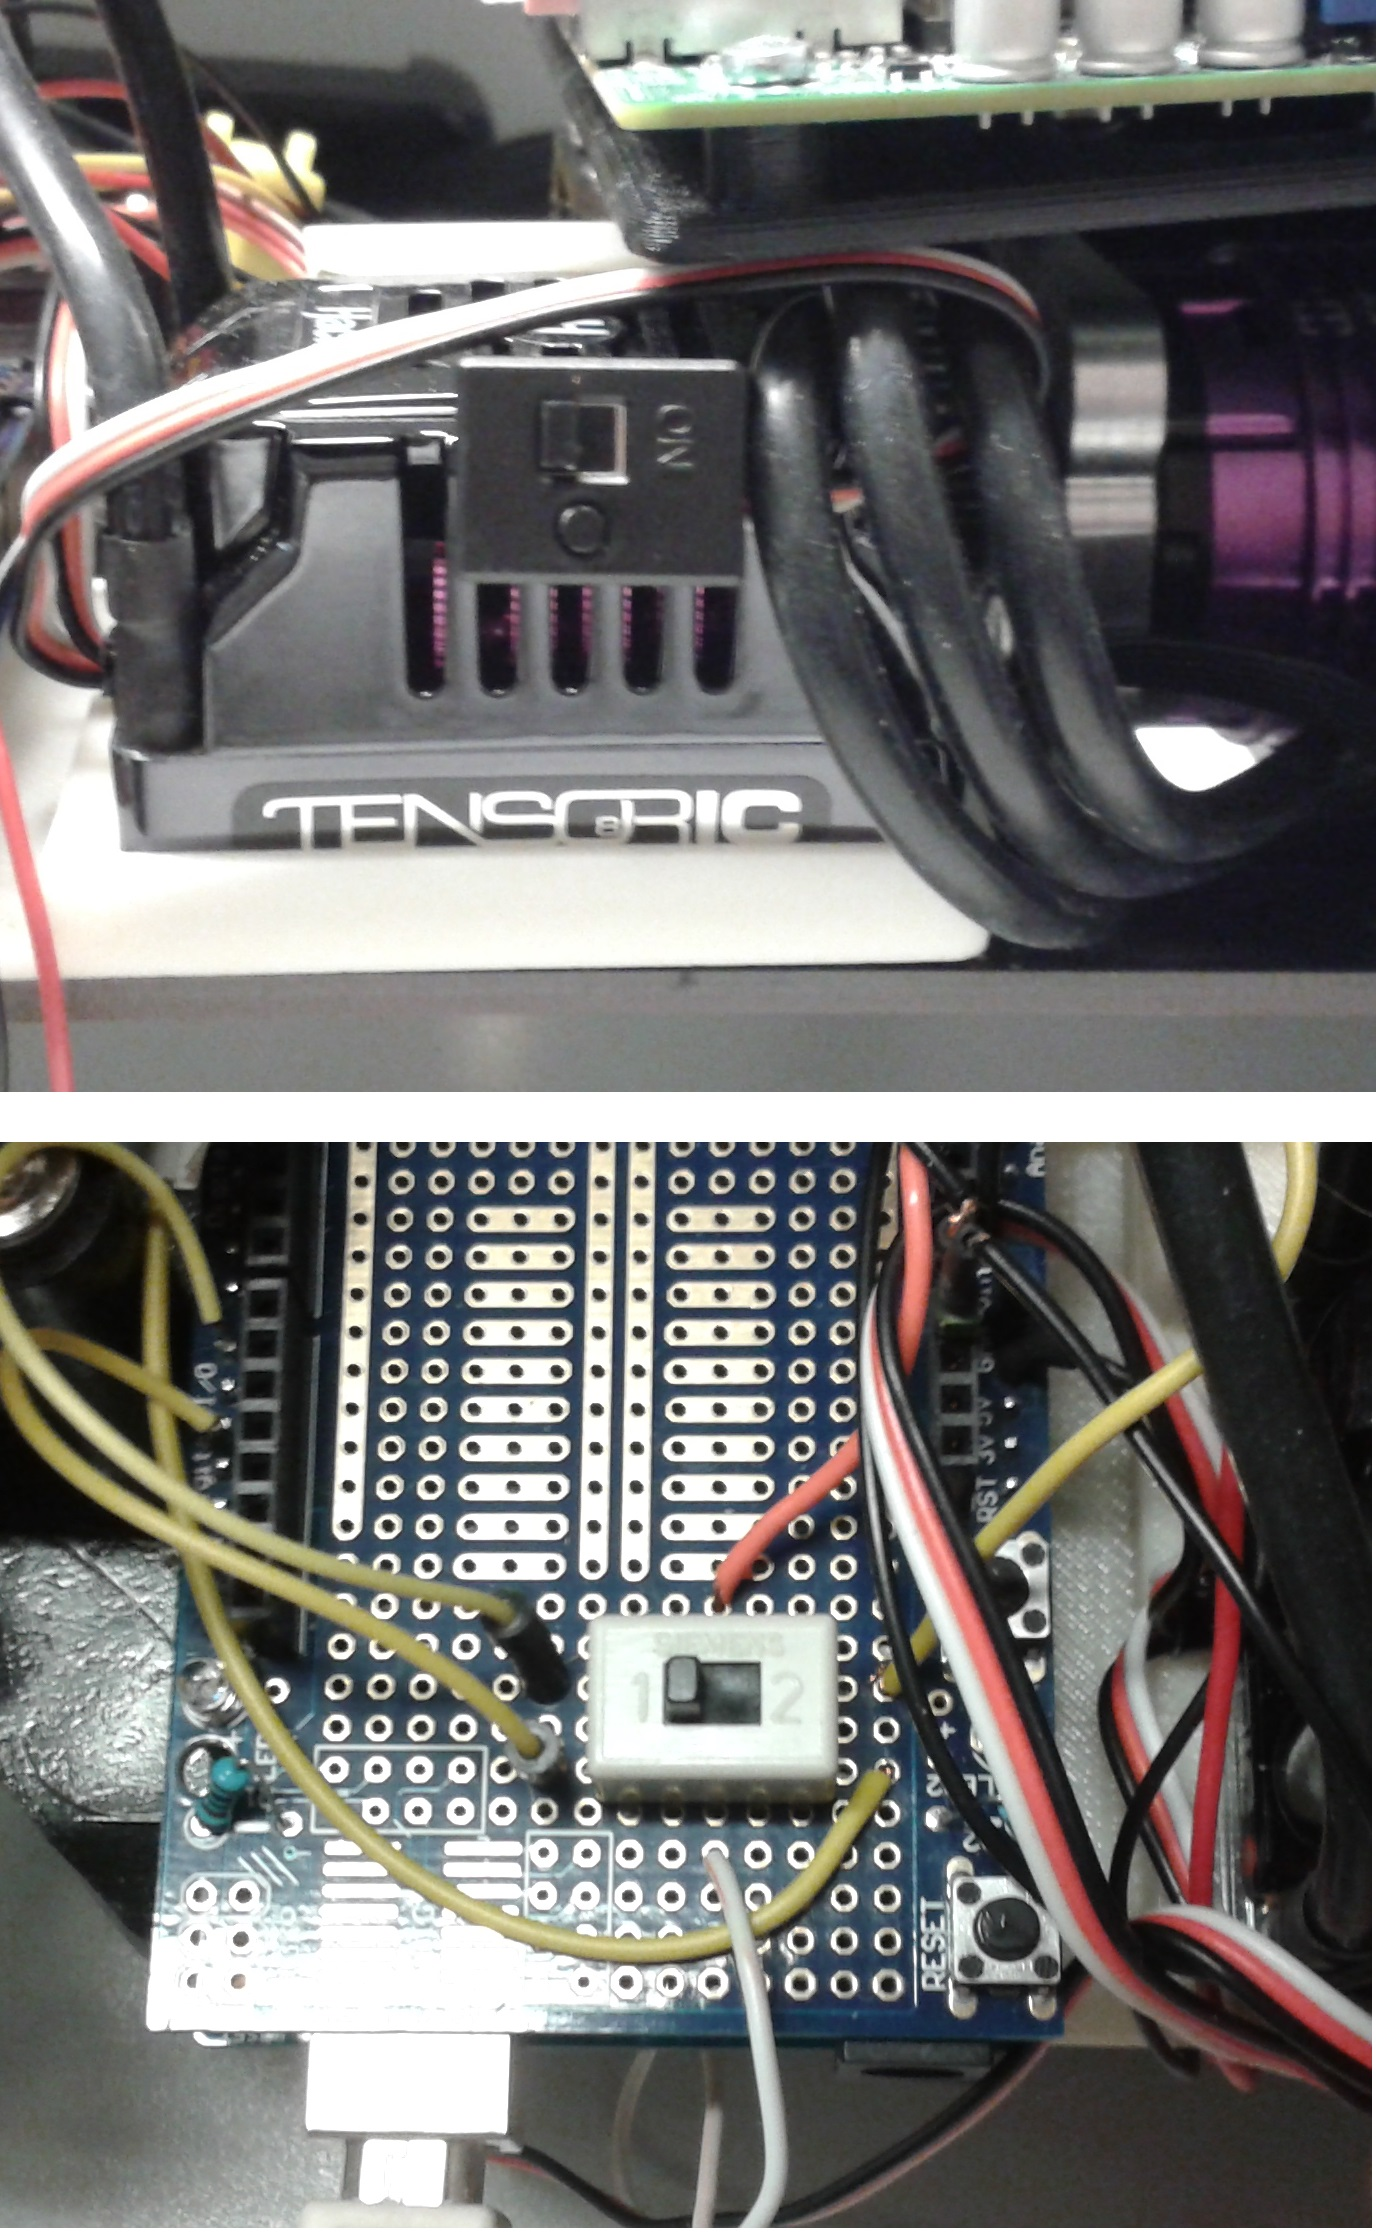
\includegraphics[width=0.33\textwidth]{switches}
		\caption{Switches for brushless motor}
		\label{fig:switches}
  \end{center}	
\end{wrapfigure} 

Power supply for the brushless motor can disconnected by a switch, which you can see in picture \reffig{switches} on the top. With the switch shown on the bottom you can select the source of the input signals for the brushless motor controller:

\begin{itemize}
\item Position 1:\\
In this position the input signal is taken from the arduino, which receives it from the ROS \texttt{/servo} topic.
\item Position 2:\\
In this positon the input signal is taken directly from the receiver for the original remote controller. This receiver is connected directly to the brushless controller. It is not connected to the Arduino or the Linux-Board in any way.
\end{itemize}



\newpage

\section{Power from external power source}
\label{setup_external}

\begin{figure}[h]
	\centering
		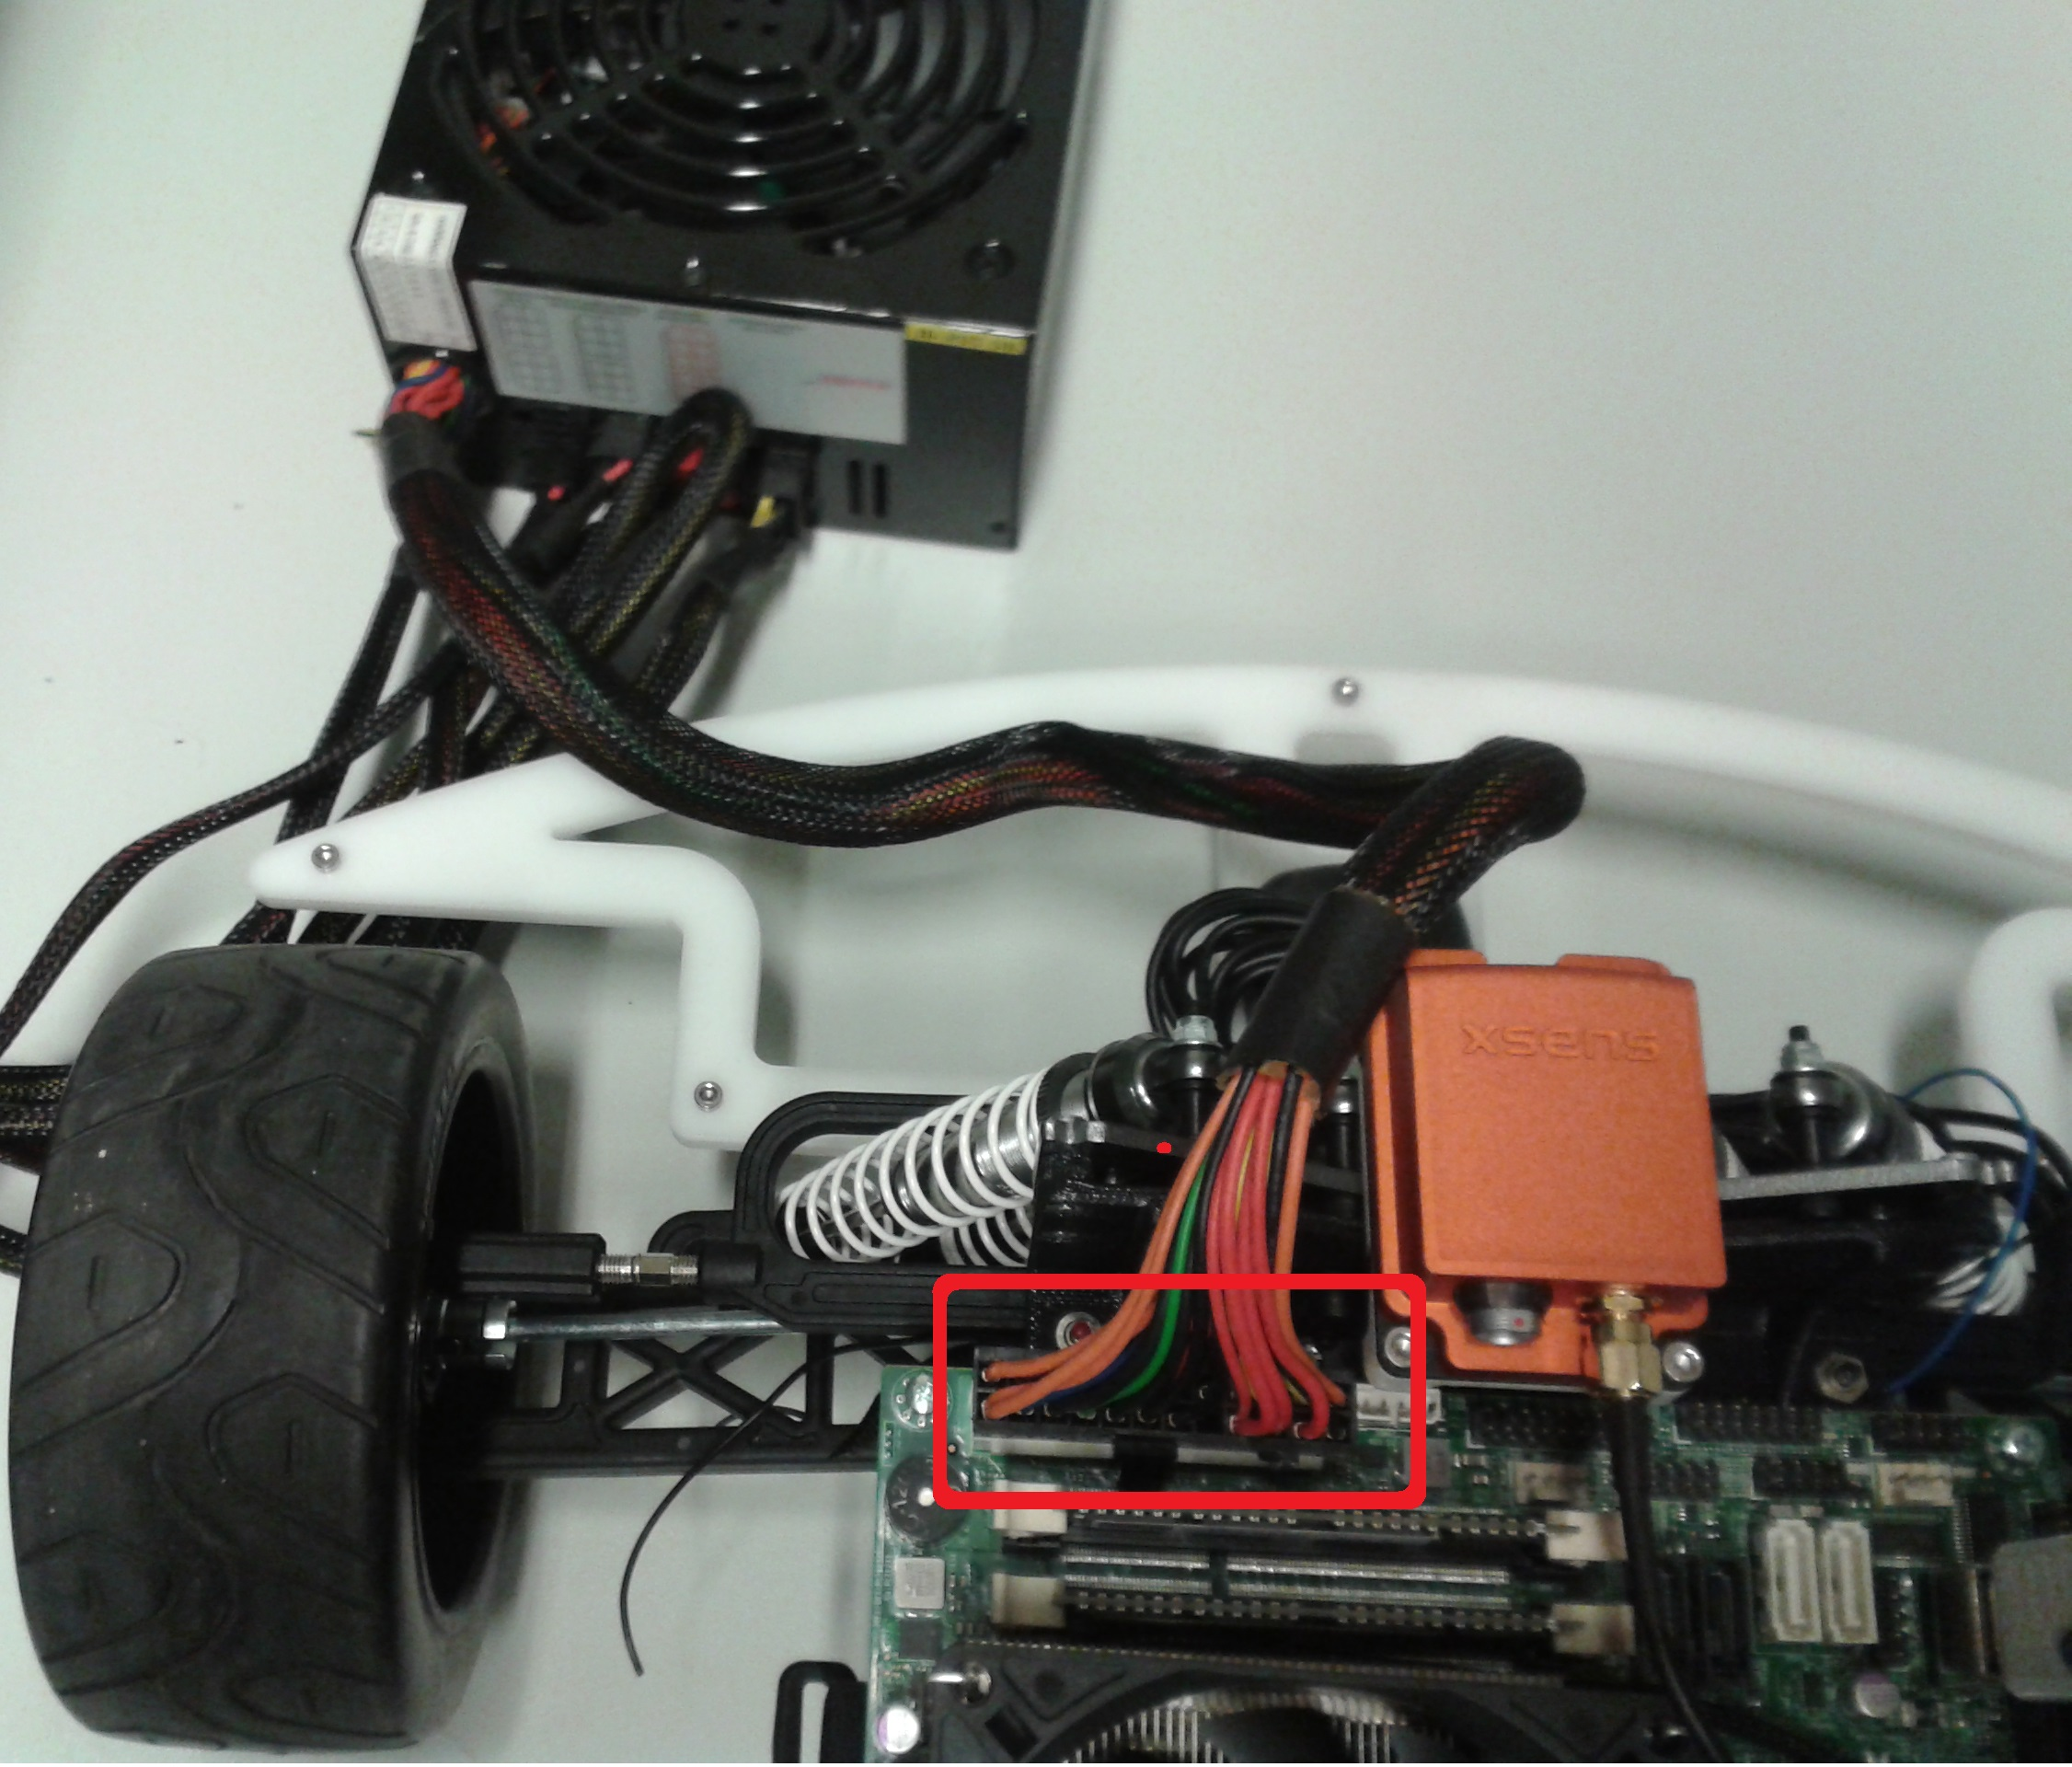
\includegraphics[width=0.55\textwidth]{ext_power}
	\caption{Connection to the external power source}
	\label{fig:ext_power}
\end{figure}
To power the board externally just connect the large 24-pin connector like it is show in picture \reffig{ext_power}. Pay attention: This will not supply the motors. These can only be powered by the battery.

\section{Power from battery}
\label{setup_battery}

\begin{figure}[h]
	\centering
		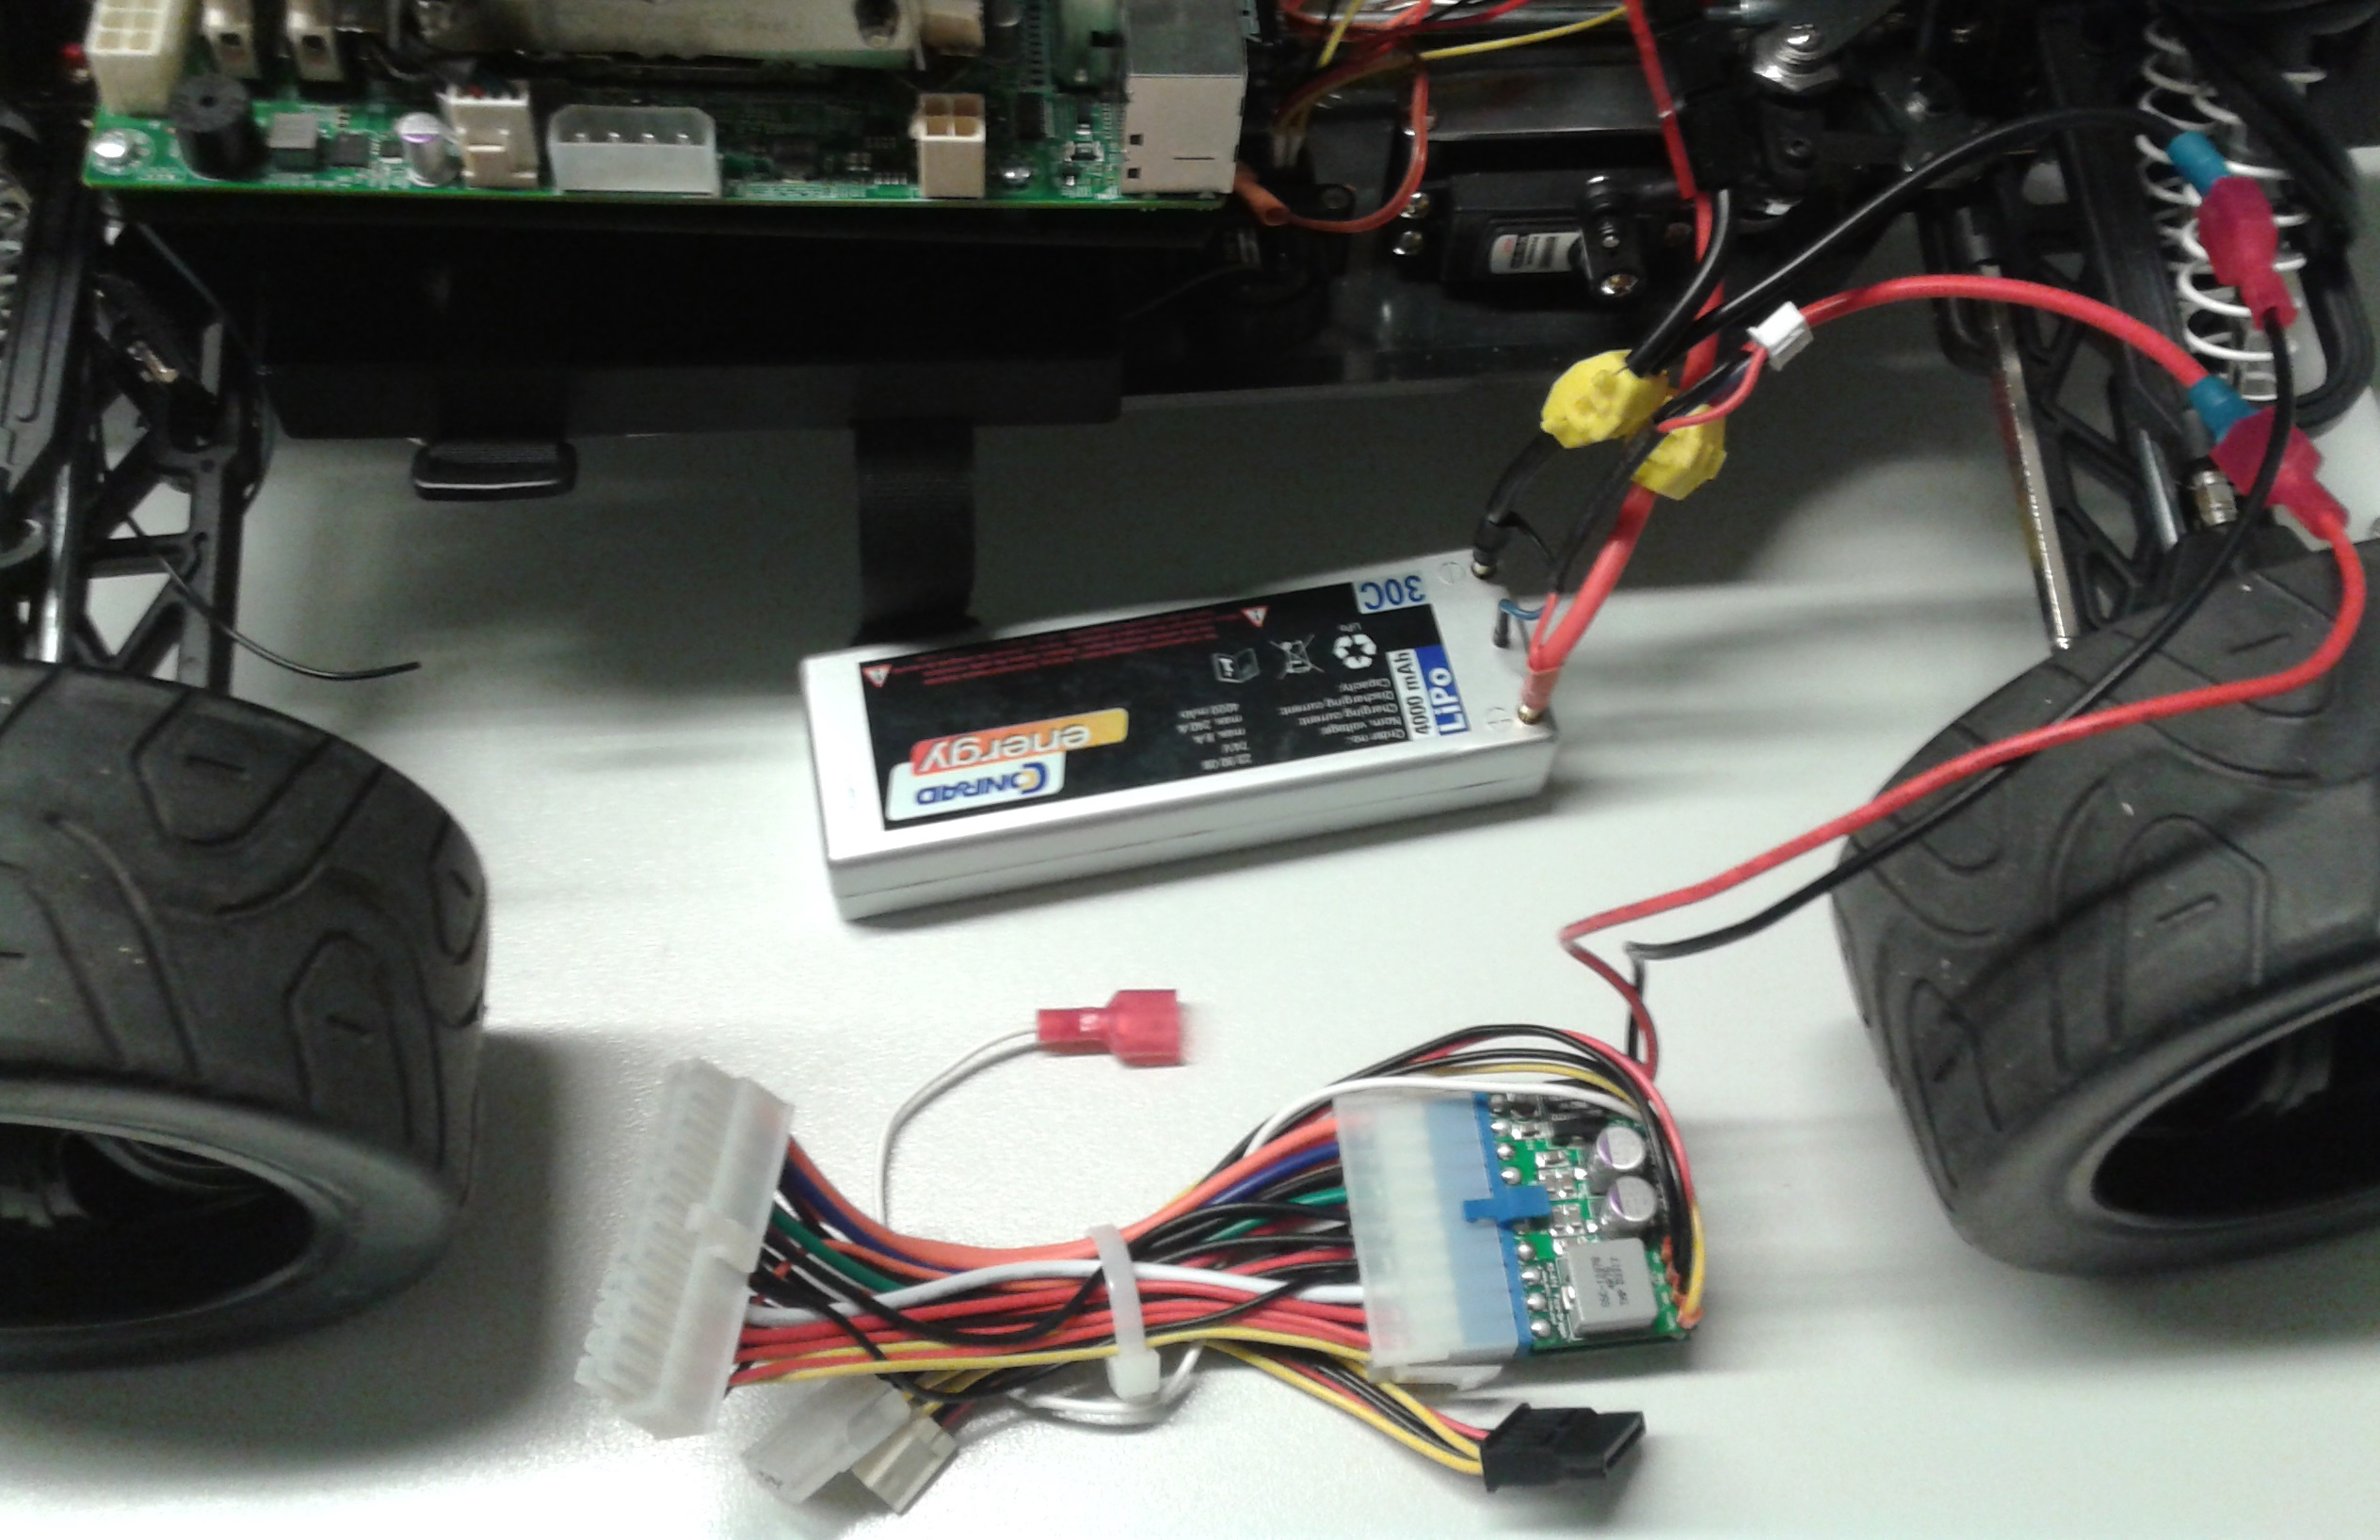
\includegraphics[width=0.55\textwidth]{batt_power}
	\caption{Connection to battery}
	\label{fig:batt_power}
\end{figure}
To supply the board from battery, there is a 12V DC-DC Converter which you can see in picture \reffig{batt_power} obove. Just connect the battery and the converter like in the picture and the plug the 24-pin connector into the board.



